\documentclass[12pt]{article} % use larger type; default would be 10pt

\usepackage[utf8]{inputenc} % set input encoding (not needed with XeLaTeX)
\usepackage[english]{babel}
%\usepackage[english]{translator}

%%% PAGE DIMENSIONS
\usepackage{geometry} % to change the page dimensions
%\geometry{a4paper} % or letterpaper (US) or a5paper or....
% \geometry{margin=2in} % for example, change the margins to 2 inches all round
% \geometry{landscape} % set up the page for landscape
%   read geometry.pdf for detailed page layout information

\usepackage{graphicx} % support the \includegraphics command and options
\usepackage[parfill]{parskip} % Activate to begin paragraphs with an empty line rather than an indent
\usepackage[cmex10]{amsmath}
\usepackage{array}
\usepackage{listings}

%%% PACKAGES
\usepackage{booktabs} % for much better looking tables
\usepackage{array} % for better arrays (eg matrices) in maths
\usepackage{paralist} % very flexible & customisable lists (eg. enumerate/itemize, etc.)
\usepackage{verbatim} % adds environment for commenting out blocks of text & for better verbati
\usepackage{subfig} % make it possible to include more than one captioned figure/table in a single float
% These packages are all incorporated in the memoir class to one degree or another...
\usepackage{fancyhdr} % This should be set AFTER setting up the page geometry
%\usepackage[2cm,headings]{fullpage}
\geometry{hmargin=2.5cm,vmargin=3cm}

\newcommand{\grimm}{$\mathcal{G}rimm$\ }
\newcommand{\Grimm}{$\mathcal{G}rimm$\ }

\pagenumbering{arabic}
\pagestyle{fancyplain}
\thispagestyle{empty}



\usepackage{ucs}
\usepackage{inputenc}
\usepackage{verbatim}
\usepackage{moreverb}
\usepackage{url}
\usepackage{amsmath,amssymb}




%%%%%%%%%%%%%%%%%%%%%%%%%%%%%%%%%%%%%%%%%%%%%%%%%%%%%%%%
%%%%%%%%%%%                                   %%%%%%%%%%
%%%%%%%%%                                       %%%%%%%%
%%%%%%%           Pour les courbes               %%%%%%%
%%%%%%%%%                                       %%%%%%%%
%%%%%%%%%%%                                   %%%%%%%%%%
%%%%%%%%%%%%%%%%%%%%%%%%%%%%%%%%%%%%%%%%%%%%%%%%%%%%%%%% 


\usepackage{tikz}
\usepackage{gnuplot-lua-tikz}

\newcommand{\MonChapitre}[2]{%
    \chapter[#1]{#2}
    \minitoc
    \addcontentsline{lof}{chapter}{%
    Chapitre \thechapter : #2 \vspace{10pt}}
}


\newcommand{\MonAnnexe}[2]{%
    \chapter[#1]{#2}
    \minitoc
    \addcontentsline{lof}{chapter}{%
    Annexe \thechapter : #2 \vspace{10pt}}
}

\usepackage{ucs}

\begin{document}

\title{\grimm: a Tool for Model Generation}
\author{Adel Ferdjoukh, Lirmm}
\date{}


\maketitle

\vspace{5cm}

\tableofcontents

\newpage

\section{What is \grimm ?}

\grimm is a tool whose the purpose it to generate models conforming to meta-models in \textit{ecore} format. It is encoded in \textit{EMF/Java}.

This tool takes as inputs a meta-model conform to \textit{ecore} and configuration data on the models to generate.

It brings two kinds of outputs. The first one is a \textit{xmi} format model which could be manipulated in eclipse and the second one is tu visual representation of this same model generated by the tool \textit{dot} of software \textit{GraphViz}.


\section{Functioning Conditions}

To make \grimm working, the computer of a user must gather the following conditions:

\begin{enumerate}
\item Install the JVM (\textit{The Java Virtual Machine}).
\item Download the \grimm archive which contains the tool and the CSP solver Abscon.
\item Install \textit{GraphViz} to be able to visualize the generated models.
\end{enumerate}

\section{Execution with simple parameters}

After gathering the functioning conditions of \grimm, you are able to spread to the execution step. To do this, you should first extract the files form the \grimm archive then follow the following steps: 


\begin{enumerate}
\item Choose one of the meta-models attached with the archive.
\item Recover from the table figure \ref{test} the root class of chosen meta-model.
\item Lunch a shell terminal and execute this following command: 

\begin{verbatim}
java -jar grimm.jar -mm=mm.ecore -rootClass=root -lb=n -ub=m -rb=l
\end{verbatim}

where:

\textbf{\textit{mm.ecore}}: File path of chosen meta-model.

\textbf{\textit{root}}: Root class of chosen meta-model.

\textbf{\textit{n}}: Instances per class lower bound.

\textbf{\textit{m}}: Instances per class upper bound.

\textbf{\textit{l}}: References upper bound (for unbounded ones).

\item Then follow instructions on the terminal. Generated models are saved in a folder named \textit{root} (different for each meta-model).

\end{enumerate}

\begin{figure}[!h]
\centering
\begin{tabular}{c|c|c}
\hline
Meta-model & File path & Root class \\
\hline
Test & test.ecore & Compo  \\
PetriNet & PetriNet.ecore & PetriNet \\
Entities \& Relashionships & ER.ecore & Schema \\
Royal and Loyal & RoyalAndLoyal.ecore & LoyaltyProgram \\
BibTex & BIBTEXML.ecore & BibtexFile \\
BMethod & BMethod.ecore & BSpec \\
Sad & Sad3.ecore & DocumentRoot \\
Diagraph & Diagraph.ecore & GraphModel \\
Business Process & BusinessProcessModel.ecore & CoumpoundTask \\
MyUML & MyUML.ecore & Model \\
Ecore & Ecore.ecore & EClass \\
Jess & jess.ecore & JessModel \\
Maps & maps.ecore & map \\
\hline
\end{tabular}
\caption{Meta-models benchmark with their root classes.}
\label{test}
\end{figure}

\begin{figure}[!h]
\centering
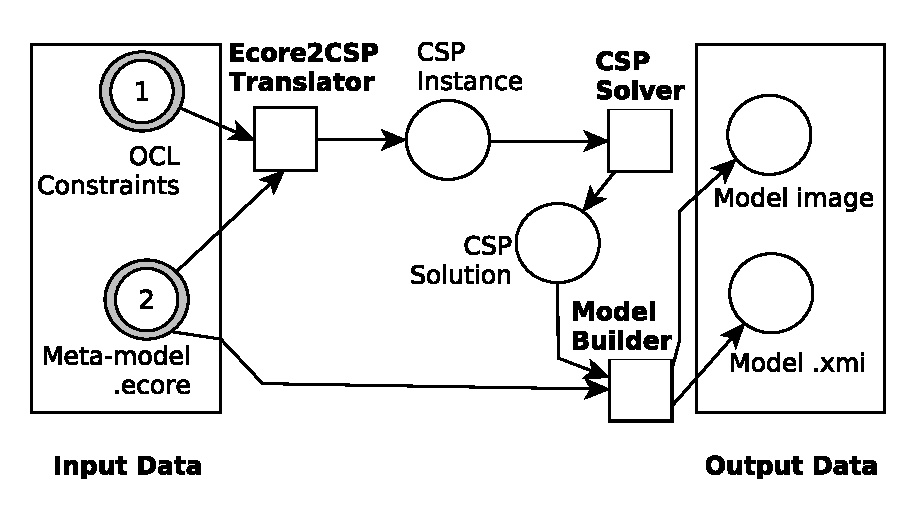
\includegraphics[scale=0.8]{precess_rdp2015EN.pdf}
\caption{Generation of models with \grimm: Process steps (simple parameters).}
\label{test1}
\end{figure} 

The steps of the process of model generation using \grimm are:

\begin{enumerate}
\item From a meta-model, generates a csp instance according to the CSP modelling of a meta-model in \cite{ferdjoukh}.
\item Use \textit{Abscon} CSP solver to solve the csp instance obtained in step 1 (\cite{abscon}).
\item Build a valid model according to the values of the solution given by the solver.
\end{enumerate}
 
These three steps are also shown in the Petri net in figure \ref{test1}. 
 
\section{Execution using a configuration file}

If you need more control and more options (for example choose a number of instances for each class separately), you can use to generate using a configuration file.

\grimm can generate a pre-filled configuration file using the following command:

\begin{verbatim}
         java -jar grimm.jar -mm=file.ecore -rootClass=root
\end{verbatim}

After that, you have to complete the filling of that generated file (root.grimm) and to lunch the following command:

\begin{verbatim}
   java -jar grimm.jar -mm=file.ecore -rootClass=root -configFile=root.grimm
\end{verbatim}

The figure \ref{configFile} gives an example of a configuration file.

\begin{figure}[!htbp]
\centering
%\includegraphics[scale=0.5]{images/map\grimm.png}
\lstinputlisting{map.grimm}
\caption{An example of a \grimm configuration file.}
\label{configFile}
\end{figure}

\begin{figure}[!h]
\centering
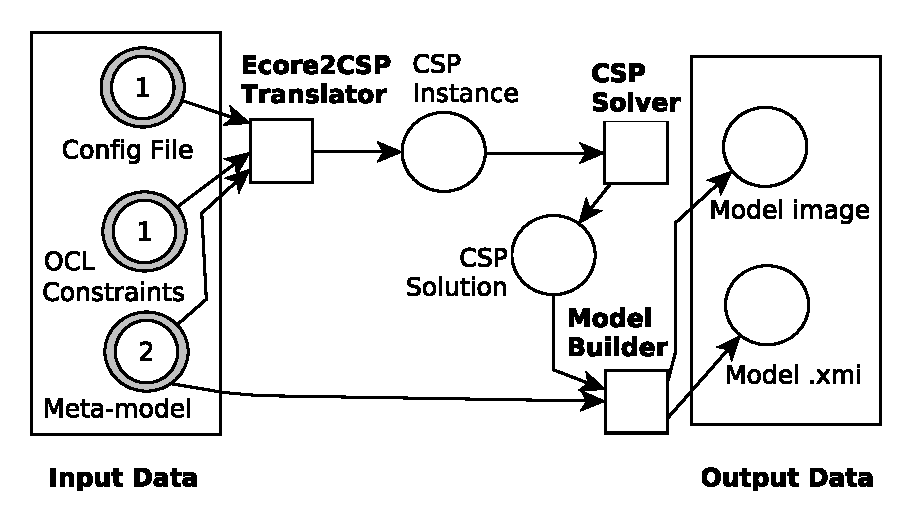
\includegraphics[scale=0.8]{precess_rdp2015EN2.pdf}
\caption{Generation of models with \grimm: Process steps (simple parameters).}
\label{process2}
\end{figure} 

\section{Other options}

To see the other options that \grimm offers, you can execute this command:

\begin{verbatim}
         java -jar grimm.jar
\end{verbatim}
 
\addcontentsline{toc}{section}{References}
\bibliography{LaBiblio}
\bibliographystyle{alpha}


\end{document}
